\section{Dataset}

The Cityscapes dataset is a large-scale dataset widely used for training and evaluating algorithms in the fields of computer vision, particularly for semantic understanding of urban street scenes. It features a collection of diverse urban street images from 50 different cities, collected across Germany and some neighbouring countries. The dataset includes over 5,000 fine annotations and 20,000 coarse annotations (see Figure \ref{fig:cityscapes}) of high-resolution images (2048$\times$1024 pixels). The fine annotations are detailed pixel-wise labels for 30 classes such as road, car, pedestrian, building, and traffic light. The detailed annotations are particularly valuable for our task where the goal is to assign a label to each pixel of the image. 

\begin{figure}[ht]
    \centering
    \begin{subfigure}{0.45\textwidth}
        \centering
        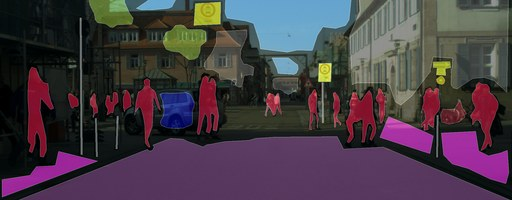
\includegraphics[width=\linewidth]{coarse_example.jpg}
        \caption{Coarse mask}
        \label{fig:sub1}
    \end{subfigure}\hfill
    \begin{subfigure}{0.45\textwidth}
        \centering
        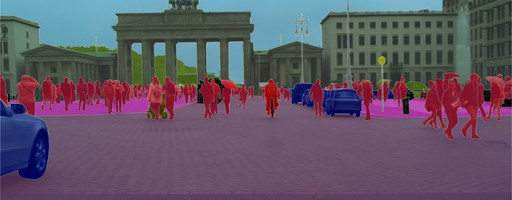
\includegraphics[width=\linewidth]{fine_example.jpg}
        \caption{Fine mask}
        \label{fig:sub2}
    \end{subfigure}
    \caption{Examples of coarse (a) and fine (b) mask annotations superimposed on the corresponding original images}
    \label{fig:cityscapes}
\end{figure}

The scenes represent a variety of seasons, daylight conditions, and weather scenarios, providing robust, real-world environments for training models that need to perform under varied conditions. This dataset has been widely used in research for developing and testing algorithms on tasks such as object detection, semantic segmentation, and instance segmentation in urban settings as well as advancing the state-of-the-art in visual perception for autonomous driving systems. The Cityscapes dataset can be accessed in the following address:
\begin{center}
\url{https://www.cityscapes-dataset.com}
\end{center}
Our particular approach in this study is to create and train at least two models; one with a basic architecture that will form our baseline and a second one where we will be exploring a more complex architecture. We are aiming to demonstrate first of all that both our models are able to perform semantic segmentation on the chosen dataset. Our second goal is to investigate how the choice of various hyper-parameters and tweaks in architecture can affect the accuracy and performance of the models. 
